\section{Description}
The Classical PSHA-based risk calculator can be used to determine loss exceedance curves under certain conditions (usually for single site loss assessments). This calculator takes the configuration information, one or several vulnerability models, information describing the assets and using hazard curves, either contained in a file or computed using a PSHA input model, computes a loss exceedance curve for each asset. Figure \ref{fig:Scheme_PSHA_calc} illustrates the architecture of this calculator:

\begin{figure}[ht]
\centering
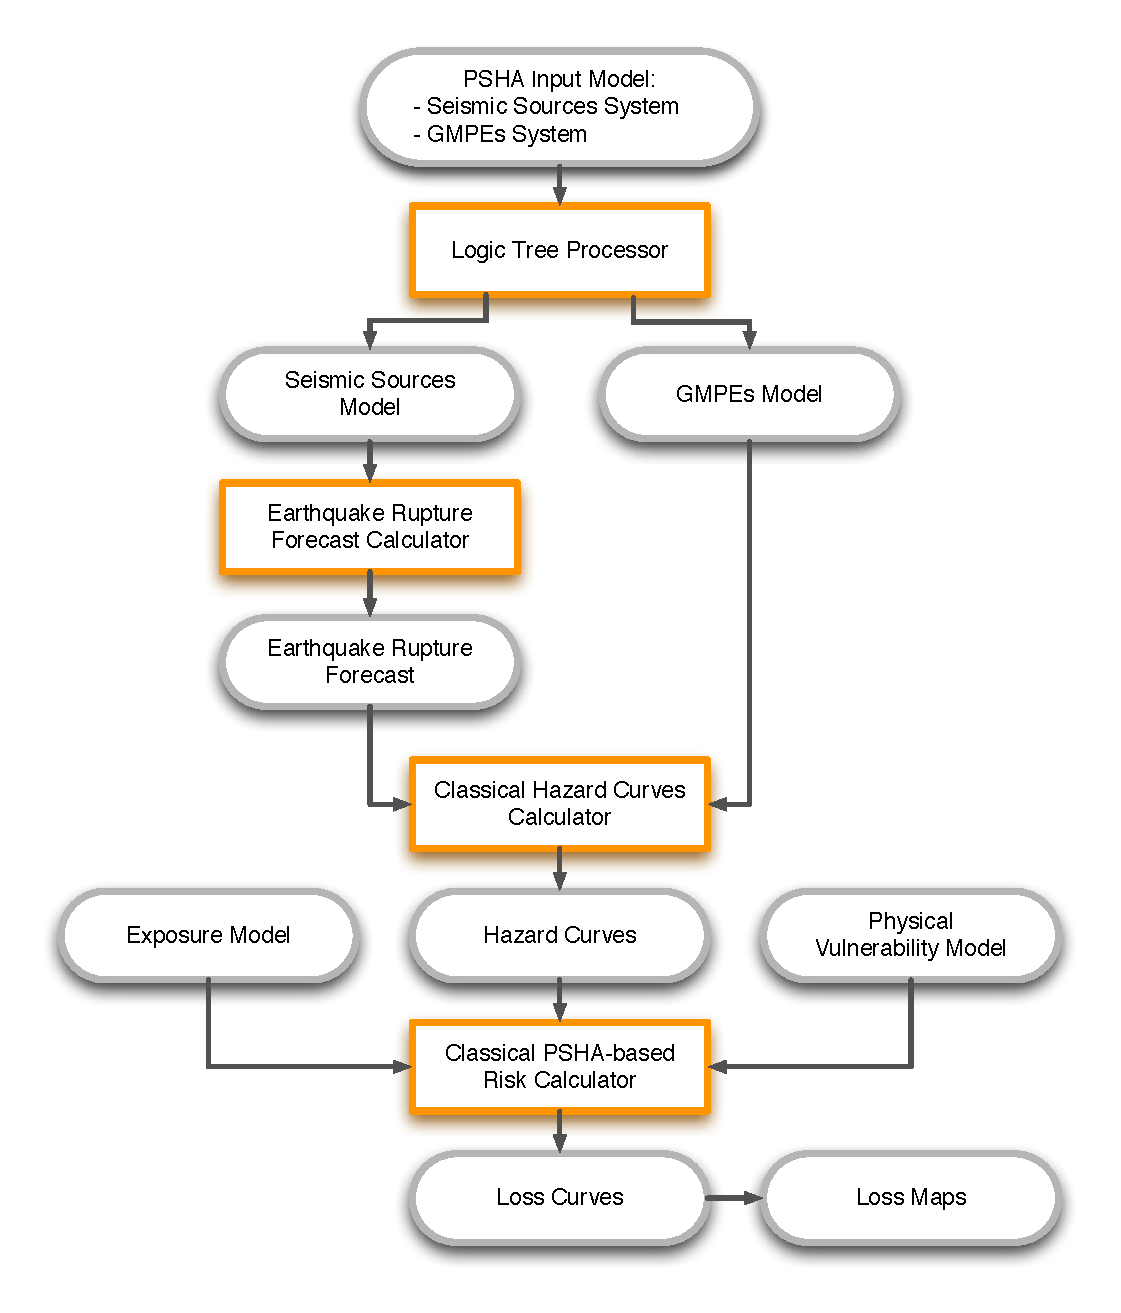
\includegraphics[width=9cm,height=9cm]{./Figures/Part_Risk/Scheme_PSHA_calc.eps}
\caption{Architecture of the Classical PSHA-based risk calculator.}
\label{fig:Scheme_PSHA_calc}
\end{figure}

\section{Calculation workflow}

\begin{enumerate}
\item By default, the hazard component of the OpenQuake engine computes the hazard curves for a set of intensity measure levels that are pre-defined in the configuration file. With the integration of the hazard and risk components in the engine, a feature is currently being implemented with the purpose of verifying that this set of values covers the range of intensity measure levels defined in the vulnerability functions. If not, the set of values in which the hazard curves are going to be computed is extended based on the minimum and maximum values of the vulnerability functions.

\item To use this calculator (to be released with V0.3), the hazard curves need first to be converted into probability mass functions (e.g. probability of occurrence of a discrete set of intensity measure levels). To do so, the engine starts by reading the intensity measure levels from the discrete vulnerability functions, and computes the central value between consecutive levels. Two consecutive values define the boundaries of the interval for each intensity measure level and by relating these limits with the hazard curve, the engine computes the corresponding probabilities of exceedance. Figure \ref{fig:ProbOccurrence} contains a discrete vulnerability function (bottom chart) and a hazard curve (top chart) in which the definition of the interval for a given intensity measure level and associated estimation of the probabilities of exceedance of each limit are illustrated. 

\begin{figure}[ht]
\centering
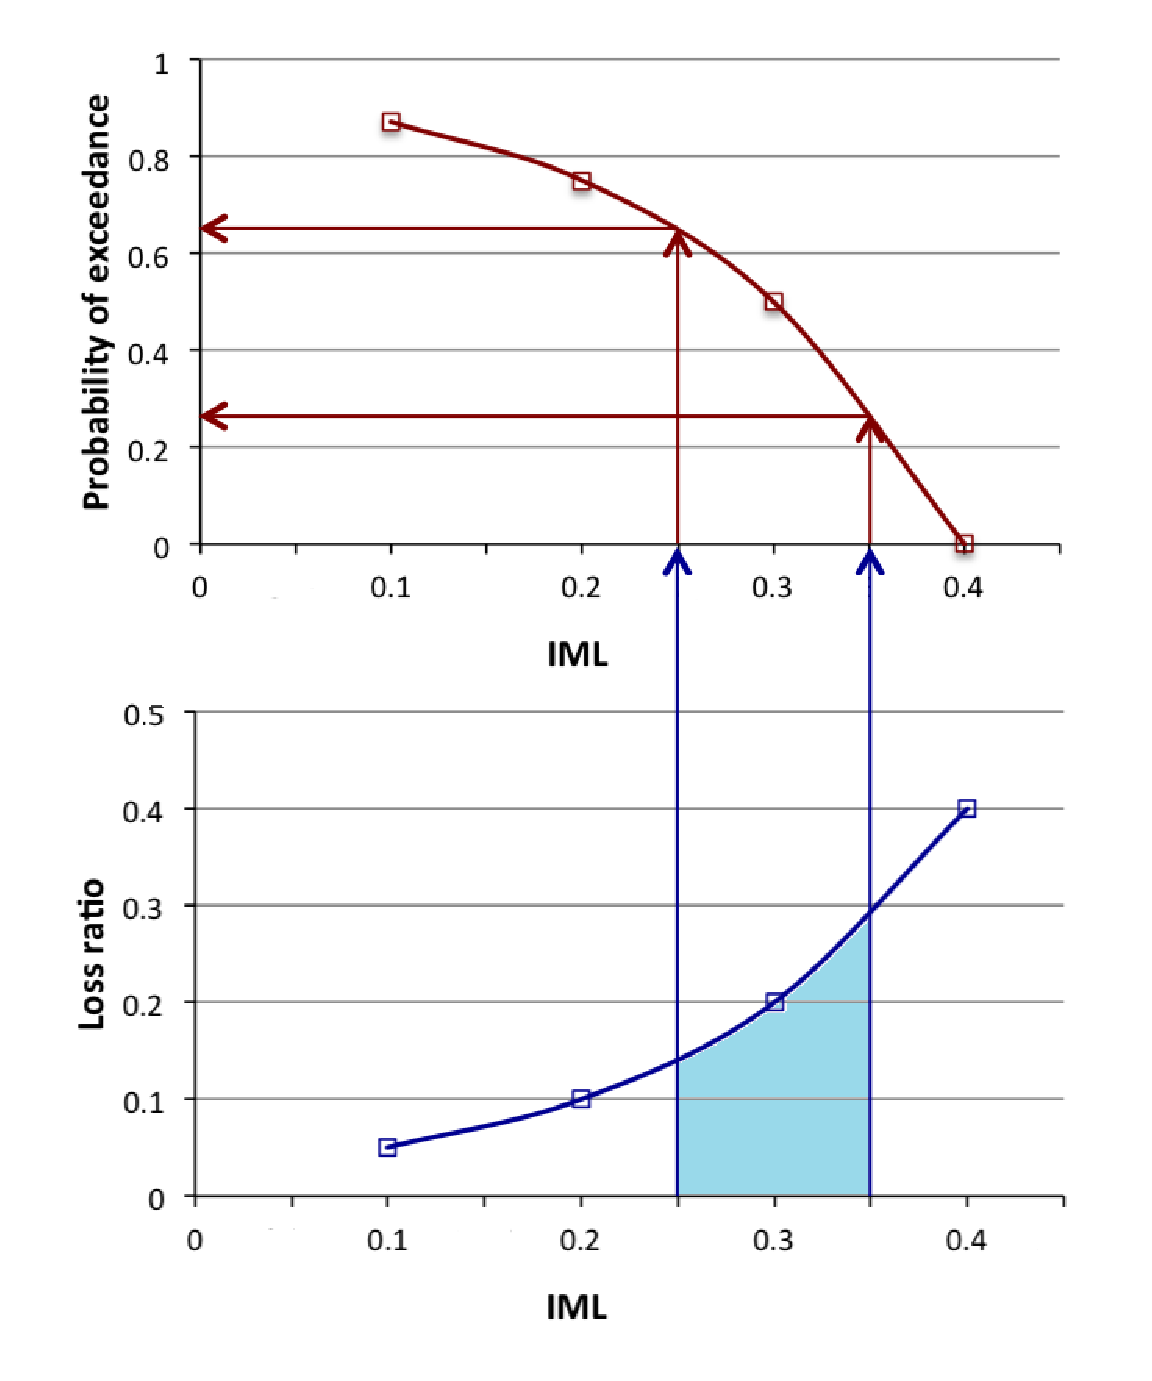
\includegraphics[width=7cm,height=8.5cm]{./Figures/Part_Risk/ProbOccurrence.eps}
\caption{Workflow to estimate the probabilities of exceedance of the boundaries of each intensity measure level.}
\label{fig:ProbOccurrence}
\end{figure}

\item The probability of occurrence of the intensity measure levels that fall within each interval can be derived by subtracting the probabilities of exceedance of the lower and upper limits, as described by the following formula:

\begin{equation}
PO= PE[lower bound]-PE[upper bound]
\end{equation}

\item The discrete vulnerability functions for each asset are converted into loss ratio exceedance matrices (e.g. matrices which describe the probability of exceedance of each loss ratio for a discrete set of intensity measure levels). These matrices have a number of columns equal to the number of intensity measure levels defined on the vulnerability function and a number of rows that can go from the number of loss ratios defined by the discrete function, up to any multiple of this number. In order to properly incorporate the probabilistic distribution of loss ratios per intensity measure level, the probabilities of exceedance should be computed not just for the loss ratios defined on the vulnerability function, but also for many intermediate values between consecutive loss ratios. Currently, following a number of sensitivity analyses, the OpenQuake engine considers 5 intermediate values between consecutive loss ratios, however, this is a parameter that will be adjustable by the user. Figure \ref{fig:LREM} contains an example of a discrete vulnerability function and the respective loss ratio exceedance matrix (in light gray):

\begin{figure}[ht]
\centering
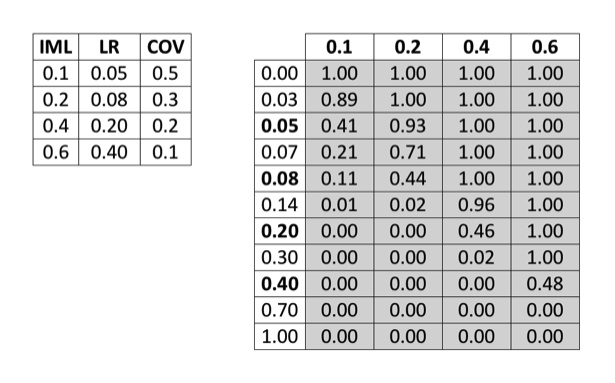
\includegraphics[width=10cm,height=6cm]{./Figures/Part_Risk/LREM.eps}
\caption{Example of a discrete vulnerability function and respective loss ratio exceedance matrix.}
\label{fig:LREM}
\end{figure}

Note that for this example only one intermediate value was considered between consecutive loss ratios and in order to consider the whole distribution of the loss ratios, the matrix was computed considering a minimum and maximum loss ratio of 0 and 1 respectively.

\item Finally, each column of the aforementioned matrix is multiplied by the probability of occurrence of the respective intensity measure level (extracted from the hazard curves) to produce a conditional loss ratio exceedance matrix.  Then, for each loss ratio the probabilities of exceedance are summed, leading to a loss ratio exceedance curve, whose set of loss ratios can be multiplied by the value of the asset given by the exposure file to obtain an absolute loss exceedance curve.

\end{enumerate}
